\documentclass[11pt, oneside]{article}
\usepackage[utf8]{inputenc}                        % utf8
\usepackage[T1]{fontenc}                           % fix font encoding
\usepackage[english]{babel}                        % language
\usepackage{titling, geometry, hyperref, fancyhdr, algorithm}
\usepackage{amsmath, amssymb, amsthm}              % ams mathematical packages
\usepackage{physics, mathtools, bm}                % extra math packages
\usepackage{graphicx, subcaption, wrapfig}         % images
\usepackage{fvextra, textcomp, CJKutf8}            % misc. text formatting
\usepackage[autostyle, english=american]{csquotes} % quotes
\usepackage[shortlabels]{enumitem}                 % lists
\usepackage{tikz, pgfplots, tikz-network}          % plots and graphs
\usepackage[noend]{algpseudocode}                  % algorithm psuedocode
\usepackage[cache=true]{minted}                    % source code
\usepackage[style=ieee]{biblatex}                  % bibliography
\geometry{a4paper}

\pgfplotsset{compat=1.17}                          % version of pgfplots
\usetikzlibrary{automata, positioning}             % markov chains

\hypersetup{
  colorlinks=true,
  urlcolor=cyan,
  linkcolor=black
}

\setminted[]{
  linenos=false,
  breaklines=true,
  encoding=utf8,
  fontsize=\normalsize,
  frame=lines,
  framesep=2mm
}

% https://tex.stackexchange.com/questions/343494/minted-red-box-around-greek-characters
\makeatletter
\AtBeginEnvironment{minted}{\dontdofcolorbox}
\def\dontdofcolorbox{\renewcommand\fcolorbox[4][]{##4}}
\makeatother

\graphicspath{{./images/}}
\addbibresource{ref.bib}

\newcommand{\emphasis}[1]{\textbf{\textit{#1}}}

\title{Keyboard LEDs and Markov Chains}
\author{Stephen Huan}
\date{January 5, 2021}

\begin{document}
\maketitle
% \tableofcontents
\section{Introduction}

The Plaid is a 4x12 ortholinear keyboard made from through
hole parts, designed by hsgw. For more information, check out
my \href{https://github.com/stephen-huan/plaid}{repository}.

\begin{figure}[h!]
  \centering
  \includegraphics[scale=0.08]{plaid}
\end{figure}

Our discussion centers around the two LEDs at the top right corner of the keyboard.
These LEDs can be programmed to turn on and off with the 
\href{https://github.com/qmk/qmk_firmware/blob/master/keyboards/dm9records/plaid/keymaps/default/keymap.c}{QMK firmware},
and while checking out the \enquote{Blinkin lights} mode
which promises to have a \enquote{random chance of state
change on each keystroke}, I saw the following C code:
\begin{minted}[label=blinkin code, framesep=1mm]{C}
case LEDMODE_BLINKIN:
  if (record->event.pressed) {
    if(rand() % 2 == 1) {
      if(rand() % 2 == 0) {
        writePinLow(led);
      }
      else {
        writePinHigh(led);
      }
    }
  }
  break;
\end{minted}

It essentially says that when a key is pressed, have a 1/2 chance of making the
state of the LED random (the C \texttt{rand()} function gives a random integer
between 0 and \texttt{RAND\_MAX}, so that integer being even or odd can be said
to have a probability of 1/2). Suppose the LED is initially on. Then the chance
it switches off when a key is pressed is a 1/2 chance for it to be random, and
a 1/2 chance that it switches off, so a 1/4 chance to be off. This is symmetric
for off to on, so the code forms a Markov chain with two states, on and off,
and a 1/4 chance to transition and a 3/4 chance to stay in the same state.

\begin{figure}[h!]
  \centering
  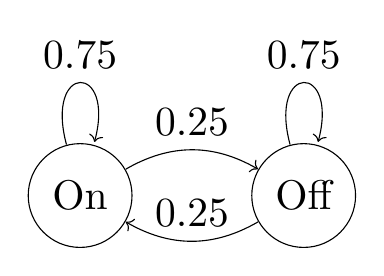
\begin{tikzpicture}[scale=1.5, transform shape]
    \node[state] (on) {On};
    \node[state, right=of on] (off) {Off};
    \path[->]
       (on) edge[bend left, auto=left]   node {0.25} (off)
      (off) edge[bend left, auto=right]  node {0.25} (on)
       (on) edge[loop above]             node {0.75} (on)
      (off) edge[loop above]             node {0.75} (off);
  \end{tikzpicture}
  \caption{Markov chain for the blinkin code.}
\end{figure}

How do we compute state changes of this Markov chain
efficiently? We can represent our current state as a 2x1
vector, which by convention will be on and then off, e.g.
\[ \vec{v} = \begin{bmatrix} p \\ 1 - p \end{bmatrix} 
\begin{matrix} p(\text{on}) \\ p(\text{off}) \end{matrix} \] 
Our transitions can then be efficiently represented as a matrix,
because the probability of being on is 
\( p(\text{on})p(\text{stay on}) + p(\text{off})p(\text{change off}) 
= 0.75p + 0.25(1 - p) \).
\[ M = \begin{bmatrix} 0.75 & 0.25 \\ 0.25 & 0.75 \end{bmatrix} \]
So pressing a key once will change our state from \( \vec{v} \) to 
\( M \vec{v} \), twice to \( M(M \vec{v}) = M^2 \vec{v} \), and \( k \)
times to \( M^k \vec{v} \). Matrix powers can be computed efficiently using
repeated squaring: squaring a matrix repeatedly generates 
\( M, M^2, M^4, \dots \), if one writes the power \( k \) in its binary form,
then it is simple to multiply these matrices to form \( k \) with 
\( O(\log k) \) matrix multiplications.
A simple implementation is \href{https://activities.tjhsst.edu/cubing/static/pdfs/cubing-lectures/EigenvaluesofPermutationMatrices/eigenvalue.pdf#page=5}{here}.

This matrix representation also gives us a nice mathematical analysis. We will
show that the \emphasis{steady-state} solution to this Markov chain is 
\( \begin{bmatrix} 0.5 & 0.5 \end{bmatrix}^T \), or the convergence of
\textit{any} initial vector to this final state given enough iterations.
If a vector \( \vec{x} \) is a steady-state solution, then multiplying by
\( M \) does not change its value. Therefore:
\begin{align*}
  M\vec{x} &= \vec{x}
  \shortintertext{Subtracting \( \vec{x} \) from both sides,}
  M\vec{x} - \vec{x} &= \vec{0} \\
  (M - I) \vec{x} &= \vec{0}
\end{align*}
This is equivalent to saying that \( M \) has an eigenvector with eigenvalue
\( 1 \). Let's solve for the eigenvectors of \( M \) and see what happens:
\begin{align*}
  \det(M - \lambda I) &=
  \begin{vmatrix} 0.75 - \lambda  & 0.25 \\ 0.25 & 0.75 - \lambda \end{vmatrix}
  = (0.75 - \lambda)^2 - \frac{1}{16} \\
  &= \lambda^2 - \frac{3}{2} \lambda + \frac{1}{2}
  = (\lambda - 1)(\lambda - \frac{1}{2}) = 0  \\
  \lambda &= \frac{1}{2}, 1 
\end{align*}
\begin{align*}
  \shortintertext{For \( \lambda_1 = \frac{1}{2} \), we find its associated eigenvector:} 
  \begin{bmatrix} 0.25 & 0.25 \\ 0.25 & 0.25 \end{bmatrix} \vec{x}_1 &= \vec{0}
  \rightarrow 0.25 x_1 + 0.25 x_2 = 0 \rightarrow x_1 = -x_2
  \shortintertext{Taking \( x_1 = 1 \),}
  \vec{x}_1 &= \begin{bmatrix} 1 \\ -1 \end{bmatrix}
  \shortintertext{Similarly, for \( \lambda_2 = 1 \):}
  \begin{bmatrix} -0.25 & 0.25 \\ 0.25 & -0.25 \end{bmatrix} \vec{x}_2 &= \vec{0}
  \rightarrow -0.25 x_1 + 0.25 x_2 = 0 \rightarrow x_1 = x_2
  \shortintertext{Taking \( x_1 = \frac{1}{2} \),}
  \vec{x}_2 &= \begin{bmatrix} 0.5 \\ 0.5 \end{bmatrix}
\end{align*}
Note that \( \vec{x}_1 \) cannot be interpreted as a probability vector because
it contains a negative value, while \( \vec{x}_2 \) is our steady-state solution.
To show that \textit{any} vector converges to the steady-state, we notice that
these two eigenvectors form an basis, since they are linearly independent and
the dimensionality of the space is 2. Thus, we can write every vector as a
linear combination of these two eigenvectors.
\begin{align*}
  \vec{v} &= c_1 \vec{x}_1 + c_2 \vec{x}_2 \\
  \shortintertext{If we multiply by \( M \),}
  M \vec{v} &= M(c_1 \vec{x}_1 + c_2 \vec{x}_2) = c_1 M \vec{x}_1 + c_2 M \vec{x}_2 \\
            &= c_1 \lambda_1 \vec{x_1} + c_2 \lambda_2 \vec{x_2} 
            =  c_1 \frac{1}{2} \vec{x_1} + c_2 \vec{x_2} \\ 
  M^k \vec{v} &= c_1 \frac{1}{2^k} \vec{x_1} + c_2 \vec{x_2} \\  
  \shortintertext{Thus, as \( k \) goes to \( \infty \), the contribution
  of \( \vec{x}_1 \) goes to 0}
  \lim_{k \to \infty} M^k \vec{v} &= c_2 \vec{x_2} = \vec{x_2} 
  \shortintertext{Since we know \( M^k \vec{v} \) is a probability vector,
  its entries must sum to 1 so \( c_2 \) must be 1.}
\end{align*}
Therefore any starting vector converges to the steady-state solution.
The proof of the remarkable fact that the distance between a vector and the
steady state halves every iteration is left as an exercise for the reader
(where \enquote{distance} is taken to be the simpler \( \ell_1 \) norm,
not the standard vector distance).

\section{Code Generalization}
Suppose we modified the probabilities in the code, that is, we made it so that
it was not necessarily a 1/2 chance of flipping a fair coin between on or off.
There are two probabilities to modify, the first which controls the probability
of flipping the coin and the second which weights the coin. It is simple
algebra to show that this code can only simulate Markov chains with transition
probabilities that sum up to less than or equal to 1. A simple Markov chain
that this code can't simulate is the one which always switches --- from on to
off and vice versa. We now consider the most general Markov chain,
characterized by two transition probabilities:

\begin{figure}[h!]
  \centering
  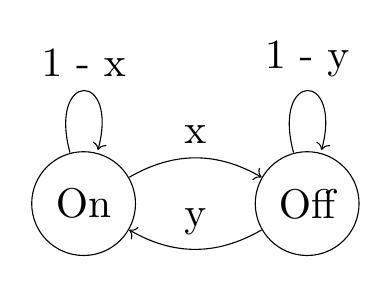
\begin{tikzpicture}[scale=1.5, transform shape]
    \node[state] (on) {On};
    \node[state, right=of on] (off) {Off};
    \path[->]
       (on) edge[bend left, auto=left]  node     {x} (off)
      (off) edge[bend left, auto=right] node     {y} (on)
       (on) edge[loop above]            node {1 - x} (on)
      (off) edge[loop above]            node {1 - y} (off);
  \end{tikzpicture}
  \caption{General Markov chain for two states.}
\end{figure}

I leave the proof that \( x \) must equal \( y \) for the steady-state to be 
\( \begin{bmatrix} 0.5 & 0.5 \end{bmatrix}^T \) for the reader. \( x = y \)
means that the Markov chain is symmetric.

We can easily simulate this in code if we have an explicit probability to
transition, and the original code is now a special case of the general code:
\begin{minted}[label=General Markov chain]{C}
  double x = 0.25; 
  double y = x;

  double p = (readPin(led)) ? x : y;
  if (rand() < p*RAND_MAX) {
    togglePin(led);
  }
\end{minted}

\subsection{Markov Chain with Random Transitions}

For our last point of analysis, we consider what happens if we randomly pick
the transition probability: not 0.25, but uniform from \( [0, 1] \):
\mintinline{C}{double x = (1.0*rand())/RAND_MAX;}

In that case, we cannot represent the Markov chain in only two states, but
it propagates forward in time like a neural network:

\begin{figure}[h!]
  \centering
  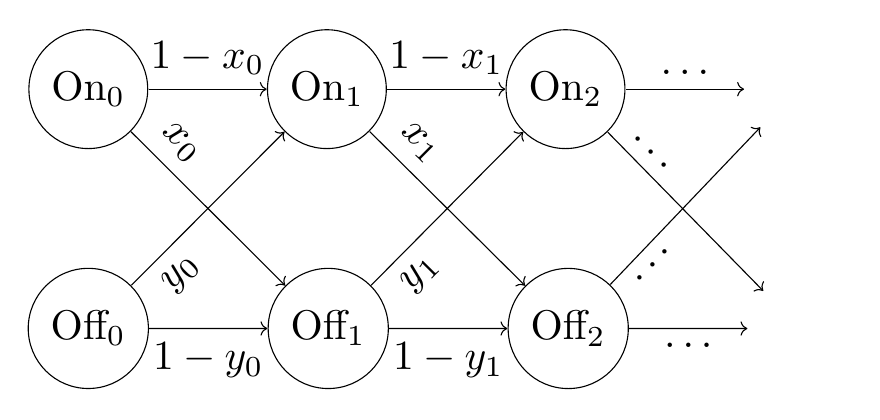
\begin{tikzpicture}[scale=1.5, transform shape]
     \node[state]                (on0) {\( \text{On}_0 \)};
     \node[state, right=of on0]  (on1) {\( \text{On}_1 \)};
     \node[state, right=of on1]  (on2) {\( \text{On}_2 \)};
     \node[state, right=of on2, draw=none]  (on3) {};
     \node[state, below=of on0] (off0) {\( \text{Off}_0 \)};
    \node[state, right=of off0] (off1) {\( \text{Off}_1 \)};
    \node[state, right=of off1] (off2) {\( \text{Off}_2 \)};
    \node[state, right=of off2, draw=none] (off3) {};
    \path[->]
       (on0) edge[above]         node {\( 1 - x_0 \)} (on1)
       (on1) edge[above]         node {\( 1 - x_1 \)} (on2)
       (on2) edge[above]         node   {\( \dots \)} (on3)
       (on0) edge[above, sloped, pos=0.2] node {\( x_0 \)} (off1)
       (on1) edge[above, sloped, pos=0.2] node     {\( x_1 \)} (off2)
       (on2) edge[above, sloped, pos=0.2] node   {\( \dots \)} (off3)
      (off0) edge[below]         node {\( 1 - y_0 \)} (off1)
      (off1) edge[below]         node {\( 1 - y_1 \)} (off2)
      (off2) edge[below]         node   {\( \dots \)} (off3)
      (off0) edge[below, sloped, pos=0.2] node     {\( y_0 \)} (on1)
      (off1) edge[below, sloped, pos=0.2] node     {\( y_1 \)} (on2)
      (off2) edge[below, sloped, pos=0.2] node   {\( \dots \)} (on3);
  \end{tikzpicture}
  \caption{Time in-homogeneous Markov Chain}
\end{figure}

We now analyze how fast it takes to converge to the steady-state solution.
Since we are sampling the transition probabilistically, the convergence is
also probabilistic. Suppose we start with a probability of \( p \) of being on,
so there is a \( 1 - p \) probability it is off. Also suppose are current 
transition probabilities are \( a \) for on to off and \( b \) for off to on.
Then after one press we have a probability of
\( (1 - a)p + b(1 - p) = (1 - a - b)p + b \) to be on. The ratio of the
distance from \( \frac{1}{2} \) before and after is then
\( \frac{(1 - a - b)p + b - 0.5}{p - 0.5} = 1 - a - b \)
with a remainder of \( \frac{-0.5a + 0.5b}{p - 0.5} \). Since we assume
\( a = b \), the remainder is zero and the distance reduction factor is 
\( |1 - 2a| \), absolute value because distance is positive. Because this is
symmetric about \( a \) and takes values uniformly between 0 and 1,
the distance reduction factor can be simplified to a
uniform random variable between \( 0 \) and \( 1 \).

Finally, we compute the probability density function of the distance by first
computing the cumulative density function, \( F_n(y) \), the probability that
after \( n \) key presses the distance is less than or equal to \( y \). To
do this we use what I like to think of as mathematical dynamic programming,
more commonly known as induction. \( F_1(y) = y \) since after one key press
the chance that the distance is less than \( y \) is if the uniform r.v. takes
a value \( \leq y \). To compute \( F_2 \), we integrate over each reduction
factor \( x \). If we want a final distance of \( y \), then any distance
less than or equal to \( \frac{y}{x} \) before multiplying by \( x \) will be
sufficient. However, we have to cap \( \frac{y}{x} \) at 1 because the distance
monotonically decreases (a distance factor larger than 1 is impossible). So
\( F_2(y) = \int^1_0 \min(F_1(\frac{y}{x}), 1) dx \). Because \( F_1(y) = y \)
and \( \frac{y}{x} \geq 1 \rightarrow y \geq x \), we split the integral into
\( \int^y_0 dx + \int^1_y \frac{y}{x} dx \) which is equal to
\( y + [y \ln x]^1_y = y - y \ln y \). Generalizing this process,
\[ F_n(y) = \int^y_0 dx + \int^1_y F_{n - 1}(\frac{y}{x}) dx 
          = y + \int^1_y F_{n - 1}(\frac{y}{x}) dx \]
and the PDF is of course \( f_n = F_n' \). Computing \( F_3 \), 
\( F_3 = y + \int^1_y (\frac{y}{x} - \frac{y}{x} \ln \frac{y}{x}) dx \).
Using integration by parts, we get \( y - y \ln y + \frac{1}{2} y \ln^2 y \).
It can be shown by induction that
\[ F_{n + 1}(y) = y - y \ln y + \frac{1}{2} y \ln^2 y - \frac{1}{6} y \ln^3 y
+ \frac{1}{24} y \ln^4 y + \dots + \frac{(-1)^n}{n!} y \ln^n y \]
Similarly, 
\[ f_{n + 1}(y) = \frac{(-1)^n}{n!} \ln^n y \] 
which comes from the interesting property that the last term of \( F_{n + 1} \),
\( \frac{(-1)^n}{n!} y \ln^n y \), derives to
\( \frac{(-1)^n}{n!} \ln^n y - \frac{(-1)^n}{(n - 1)!} \ln^{n - 1} y \), so if
\( F_{n} \) derives to \( \frac{(-1)^n}{(n - 1)!} \ln^{n - 1} y \)
(the inductive hypothesis), the two terms cancel when
they are added together, leaving \( f_{n + 1} \).

What are the characteristics of this series? It is hard to analyze
mathematically, but simple numerical experimentation shows that the expected 
distance decreases exponentially as the number of key presses increases.
That is, if one is  99\% sure that they are within 0.01 of the steady-state,
it is an linear amount of additional key presses to be 99.9\% sure or to be
within 0.001 of the steady-state. Thus, it is efficient to be \enquote{probably 
approximately correct}. Compare this to the original code which guarantees
halving of the distance to the steady state every iteration --- there are no
probabilities, and it is easy to see that it takes a linear number of key
presses to increase the number of significant figures one is from the
steady-state. Such is the cost of probabilistic algorithms.

\subsection{Implementation}

An implementation of the random transition Markov chain with some nice ASCII is
\href{https://github.com/qmk/qmk_firmware/blob/master/keyboards/dm9records/plaid/keymaps/stephen-huan/keymap.c}{here}.
Lastly, we verify that the math we did was correct. We simply do \( 10^5 \)
iterations with a computer to get a histogram of the distances, and compare
to our theoretical result.

\begin{figure}[h!]
  \centering
  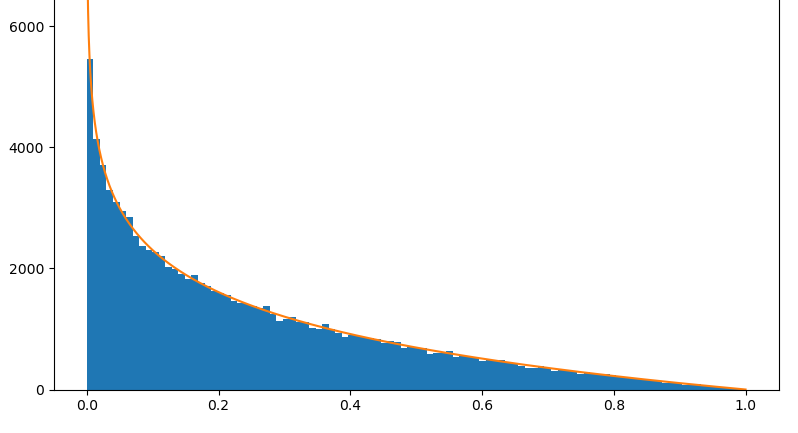
\includegraphics[scale=0.6]{graph}
  \caption{Monte Carlo simulation (in blue) versus
  theoretical computation (in orange)}
\end{figure}

The Python code is on the next page.

\begin{minted}[label=simulation]{python}
import numpy as np
import matplotlib.pyplot as plt
from scipy.special import factorial

def sample(l: int=1) -> float:
    """ Draws a random distance factor. """
    d = 1
    for i in range(l):
        p = np.random.rand()
        d *= abs(1 - 2*p)
    return d

def prob(d, c) -> int:
    """ Iters until the chance that the distance is <= d is >= c """
    # initial distance starts at 1/2
    d *= 2
    i = 1
    p = d
    lg = np.log(d)
    while p < c:
        p += abs(d*np.power(lg, i)/factorial(i))
        i += 1
    return i

print(prob(0.01, 0.99))

N = 10**5
l = 2
data = [sample(l) for i in range(N)]

fig = plt.figure()
plt.hist(data, 100)
x = np.linspace(0, 1, num=N)
plt.plot(x, -1000*np.log(x))
plt.show()
\end{minted}

% \printbibliography
\end{document}
